\documentclass[reprint,nofootinbib,...]{revtex4-1} 
%\documentclass[draft,nofootinbib,...]{revtex4-1} 
\usepackage{amsmath}%
\usepackage{amsthm,amssymb}
\usepackage{graphicx}
\usepackage{epstopdf}
\usepackage{xcolor}
\usepackage{algcompatible}
\usepackage[size=small]{caption}
\usepackage{etoolbox}
\usepackage{booktabs}
\usepackage{multirow}
\usepackage[utf8]{inputenc}
\usepackage[colorinlistoftodos]{todonotes}

\usepackage[hyperfootnotes=true]{hyperref}
\hypersetup{
 colorlinks=true,
 citecolor=blue,
 linkcolor=blue,
 urlcolor=blue}
 
% some placeholds for various parameters of the network, dataset, experiments, etc
\newcommand{\nconst}{128}       % number of jet constituents
\newcommand{\ptcut}{1.3}           % leading jet pT cut
\newcommand{\nlayerCLS}{3}     % number of layers in the target classifier
\newcommand{\nunitsCLS}{256} % number of units per layer
\newcommand{\ntrain}{145k}       % number of training samples
\newcommand{\nval}{26k}            % number of validation samples

\newcommand{\aucCLS}{0.88}    % validation AUC of benchmark classifier

% convenience defs
\newcommand{\pt}{p_\mathrm{T}} % needs mathmode

%%% ----------------------------------------------------------------------
\begin{document}

%Title of paper
\title{AI Safety for High Energy Physics}

\author{Benjamin Nachman}
\email{bpnachman@lbl.gov}

\affiliation{Physics Division, Lawrence Berkeley National Laboratory, Berkeley, CA 94720, USA}

\author{Chase Shimmin}
\email{chase.shimmin@yale.edu}

\affiliation{Department of Physics, Yale University, New Haven, CT 06511, USA}


\begin{abstract}

The field of high-energy physics (HEP), along with many scientific disciplines, is currently experiencing a dramatic influx of new methodologies powered by modern machine learning techniques.
Over the last few years, a growing body of HEP literature has focused on identifying promising applications of deep learning in particular, and more recently these techniques are starting to be realized in an increasing number of experimental measurements.
%% CS: Not sure if it's a good idea to have references in the abstract? Also, maybe we shouldn't jump right in with jargon like "low-level featuers".
%Since the first application of deep learning on `low-level' features for classification in high-energy physics (HEP)~\cite{Baldi:2014kfa}, there has been a rapidly expanding literature on the adaptation of industrial deep learning techniques as well as the development of novel methods.
The overall conclusion from this impressive and extensive set of studies is that rarer and more complex signatures can be identified with the new set of powerful tools from deep learning.  However, there is an unstudied systematic risk associated with combining the traditional HEP workflow and deep learning with high-dimensional data.
In particular, calibrating and validating the response of deep neural networks is in general not experimentally feasible, and therefore current methods may be biased in ways that are not covered by current uncertainty estimates.
By borrowing ideas from AI safety, we illustrate these potential issues and propose a method to bound the size of unaccounted for uncertainty.
In addition to providing a pragmatic diagnostic, this work will hopefully begin a dialogue within the community about the robust application of deep learning to experimental measurements and searches.
\end{abstract}

\date{\today}
\maketitle

%%%%%%%%%%%%%%%%%%%%%%%%%%%%%

\section{Introduction}
%%% Note: having a hard time striking a balance between explaining how we do analysis at the LHC, so that other fields can understand the problem,
%%% vs, keeping this short and generic enough to underscore how it applies other fields.
Collider-based high-energy physics (HEP) relies critically on sophisticated simulations which model length scales from sub-nuclear reactions all the way to macroscopic detector-length scales in order to connect fundamental theories to experimentally-observable quantities.
These simulations are highly sophisticated, but are an approximation to nature and therefore systematic mismodeling must be accounted for by calibrating to data.
Searches for physics beyond the standard model generally depend on placing bounds on anomalous disagreement between simulated Standard Model (SM) predictions and experimental observations; hence, it is essential that any anomalies that may appear due to mismodelling are understood precisely.

In the traditional paradigm, a discriminating observable $m$ is used to isolate a region $s$ of phase space called the \textit{signal region}, where the expected rate of a hypothetical signal is large relative to the background.
The sensitivity of this approach is generally related to the relative rates of the signal and background, as well as the precision with which the background may be estimated.
In order to constrain the latter, a separate region $c$ of phase space is defined, where contributes from new physics are expected to be negligible, providing a pure sample of SM background processes.
In this \textit{control region}, the simulation is adjusted to match the observed data (for example, by scaling an unknown normalization, or by constraining nuisance parameters of the simulation model).
Then using the adjusted simulation, a prediction for the background rate may be extrapolated into the signal region.

%In the traditional paradigm, a discriminating observable $m$ is used to isolate a region of phase space $m<c$ where contributions from new physics are expected to be small compared with the SM background processes.
%In this \textit{control region}, the predicted cross-section is scaled to match the data and then the scaled differential cross-section from simulation is used to estimate the Standard Model contribution in a \text{signal region} with $m\gg c$.
%Theoretical uncertainties on the extrapolation are estimated by repeating this procedure with a variety of simulations.

Traditionally, a signal and control regions would be defined by applying selective criteria on physical observables, such as particle momenta or topological structure of an event.
However, it is often the case that several different observables, perhaps in some complicated relationship, are useful for isolating signal and background processes.
A typical application of machine learning in HEP is to automate the construction of signal and control regions by reformulating the task as an optimization problem; for example, a binary classifier may be trained on simulation to predict signal-like and background-like events.
While this has been done for years~\cite{} using ``shallow'' classifiers such as BDTs~\cite{}, the success of these methods have generally been very sensitive to the exact observable features selected as input to the classifier, incurring a significant amount of effort towards ``feature engineering'' to identify useful \textit{high-level} observables.

With the more recent introduction of deep learning methods, it has become possible to construct increasingly elaborate regions using higher-dimensionality input features.
Perhaps surprisingly, it has been shown~\cite{Baldi:2014kfa,deOliveira:2015xxd,Baldi:2016fql,Guest:2016iqz} that when provided with \textit{low-level} features (\textit{i.e} observables that are minimally processed using physical intuition), deep neural networks are able to automatically learn to exceed the performance of networks trained on the physically-motivated high-level features.

%Deep learning offers a new set of tools in HEP for seeking out new particles using high-dimensional, low-level information~\cite{Baldi:2014kfa,Larkoski:2017jix,Radovic:2018dip,Guest:2018yhq}.
%A growing number of searches at the Large Hadron Collider are using deep learning methods to construct $m$.
%The control region method is the baseline approach for estimating the SM background in the nascent deep learning era.

Increasingly, LHC experimentalists are taking this message to heart, with searches starting to emerge~\cite{Andrews:2018nwy,Andrews:2019faz,more??} which are built around deeper networks with high-dimensional and low-level (HDLL) input feature spaces.
This trend is also seen in related fields such as neutrino physics, where various TPC detector experiments are moving towards deep learning on very low-level data to replace conventional event reconstruction methods~\cite{Acciarri:2016ryt,Delaquis:2018zqi}.


%A potential problem of the control region method with deep learning is that the calibration procedure may not sufficiently probe the high dimensionality of the feature space.  For example, if $\mathcal{O}(1000)$ dimensions are used for training a neural network, but only $\mathcal{O}(1)$ simulation variations are considered for the uncertainty on the calibration (as is common), then the prediction in the signal region may be incorrect: the uncertainty may be much smaller than the potential bias.

A potential problem arises when combining deep learning on HDLL features to the conventional simulation-based analysis paradigm.
As noted above, physics simulation will in general differ from real observables, and while we are able to mitigate this effect by calibrating and validating certain physical observables (such as reconstructed particle states) in order to evaluate systematic effects, it may be experimentally infeasible to calibrate or even validate simulations of HDLL features.
Moreover, recent developments in the area of AI safety have demonstrated that when neural networks operate on high-dimensional input spaces, it is generically possible to get arbitrary degradation of network performance by applying subtle deviations to the input features.


%This work uses methods from AI safety to diagnose the sensitivity of the current methodology to under-constrained feature spaces.
%In particular, a common high-dimensional classification problem from jet physics is used to illustrate the sensitivity to small perturbations in measured particle properties and also to devise a sensitivity diagnostic with a directed adversarial attack.
%Certainly nature is not evil, but without any good estimate of high dimensional correlated uncertainty, this bound can be used to demonstrate robustness. 

To illustrate this problem, we implement an adversarial attack that demonstrates small perturbations in detector-level measurements can have drastic effects on the performance of a neural network trained to identify signal-like events.
This adversarial procedure can be conceptualized as a sort of \textit{demon}~\cite{TheLordKelvin} which intercedes between a physical process and the observation of that process, in such a way as to maximally confound a neural network while being minimally noticeable by experimental standards.
While certainly no such demon exists, we propose a procedure based on this method as a diagnostic tool to evaluate the worst-case sensitivity of a deep network architecture to uncertainty in high-dimensional correlations.
This bound may then be used either to demonstrate the a given network architecture is manifestly robust against HDLL systematics, or as a guiding metric to aid in the future development of more robust networks.

\section{Benchmark Problem}

As one of the first examples of high-dimensional deep learning in high-energy physics, jet classification~\cite{Larkoski:2017jix} is used as the prototypical example.
Jets are collimated sprays of particles resulting from high energy quark and gluon fragmentation, which are clustered~\cite{Cacciari:2008gp} into groups that approximate physical states in the original hard scattering process.
As such, one can represent a jet $J_i$ by the momenta of its $N_i$ constituent particles $\{(p_{T,ij},\eta_{ij},\phi_{ij})\}\in\mathbb{R}^{3N_i}$, ignoring particle masses and other quantum numbers\footnote{explain what $p_\mathrm{T}$, $\eta$, $phi$ are}.
A typical problem is to identify whether a jet originated from a quark/gluon state, or by the decay of some massive particle.
We use the dataset simulated in~\cite{gregor_kasieczka_2019_2629073}, in which the background process is generic quark and gluon scattering, while the signal process is comprised of hypothetical massive particles with masses of $100$, $500$, or $3500\ \mathrm{GeV}$ which decay into quark pairs.
Pythia~8~\cite{Sjostrand:2006za,Sjostrand:2007gs} and Delphes 3.4.1~\cite{deFavereau:2013fsa} are used to simulate the scattering process and detector response, respectively.
Jets are clustered using Fastjet~\cite{Cacciari:2011ma,Cacciari:2005hq} vis pyjet~\cite{noel_dawe_2019_2672944} implementing the anti-$k_t$ algorithm with radius parameter $R=1$~\cite{Cacciari:2008gp}.
Each event is required to have a jet with $p_\mathrm{T} > 1.3\ \mathrm{TeV}$, and only the leading jet is considered.

Hence, we first train a benchmark classifier network $f$ which will be the target of our adversarial attack.
The network takes as input a $\nconst\times3$ tensor $x$ corresponding to the constituent momenta of a jet.
Jets with more than $\nconst$ constituents are truncated by dropping the lowest-$\pt$ constituents; the tensors are padded with zeros for jets with fewer constituents.
The inputs are fed into a fully-connected neural network with \nlayerCLS\ hidden layers, each with \nunitsCLS\ units and ReLU activation.
The output layer is a single neuron with a sigmoid activation, and the loss function is the binary crossentropy between the network output $f(x)$ and the target labels $y$, in which $y=0$ corresponds to background events, and $y=1$ corresponds to signal.

The classifier network is trained with the Adam~\cite{adam} optimizer on \ntrain\ events with a 50\% signal/background split, and validated on \nval\ events.
Training proceeds until the validation loss begins to diverge from the training loss, resulting in a final network with a validation AUC of \aucCLS.

\section{Methods}
To demonstrate the sensitivity of existing methods to small perturbations to the input particles in high dimensions, a fast gradient sign method (FGSM) is deployed~\cite{DBLP:journals/corr/GoodfellowSS14}.  The idea is that individual jets are perturbed $J\mapsto \delta J_i$ based on the gradient of the classification loss.  Each jet is independently modified, which is an unlikely scenario for high-dimensional mis-modeling, but is a robust indication of a classifier's sensitivity to fixed small perturbations.  A universal modifier is discussed later.  A deep neural network $f(J_i)\mapsto [0,1]$ is trained in the usual way $f=\text{argmin}_{f'}\mathcal{L}(F'(J),y)$, $y\in\{0,1\}$, where $\mathcal{L}$ is the loss function (in this case, cross-entropy).  Networks are trained with Keras~\cite{keras} using the Tensorflow~\cite{tensorflow} backend and optimized using Adam~\cite{adam}.  To compare the sensitivity of a deep neural network trained directly on the natural high-dimensionality with traditional methods, a second network is trained whose first layer is a ratio of energy correlation functions~\cite{Larkoski:2013eya} known as $D_2$~\cite{Larkoski:2014gra}.

The FGSM modification is then given by

\begin{align}
\label{eq:FGSM}
f(J_i+\epsilon\times\text{sign}(\Delta_J(\mathcal{L}(f,J))|_{J=J_i}),
\end{align}

\noindent where $\epsilon=(\epsilon_{p_T},\epsilon_\eta,\epsilon_\phi)^N, \epsilon_i\ll1$ is a small perturbation.  In the example below, $\epsilon=(2,20,20)\times 10^{-4}$.  The process illustrated in Eq.~\ref{eq:FGSM} is repeated $N=10$ times.  Figure~\ref{fig:FGSM} blah...

\begin{figure}[h!]
\centering
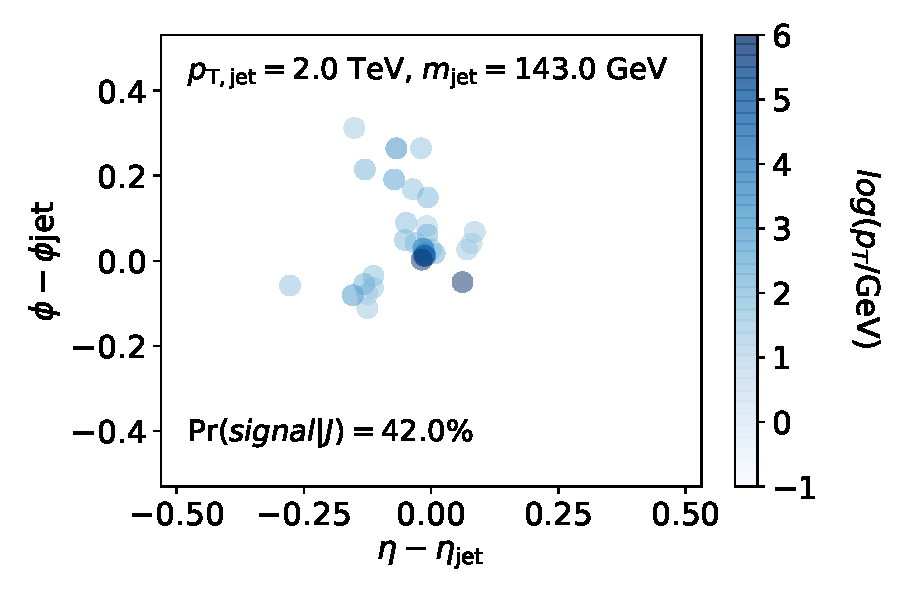
\includegraphics[width=0.15\textwidth]{figures/panel_1.pdf}
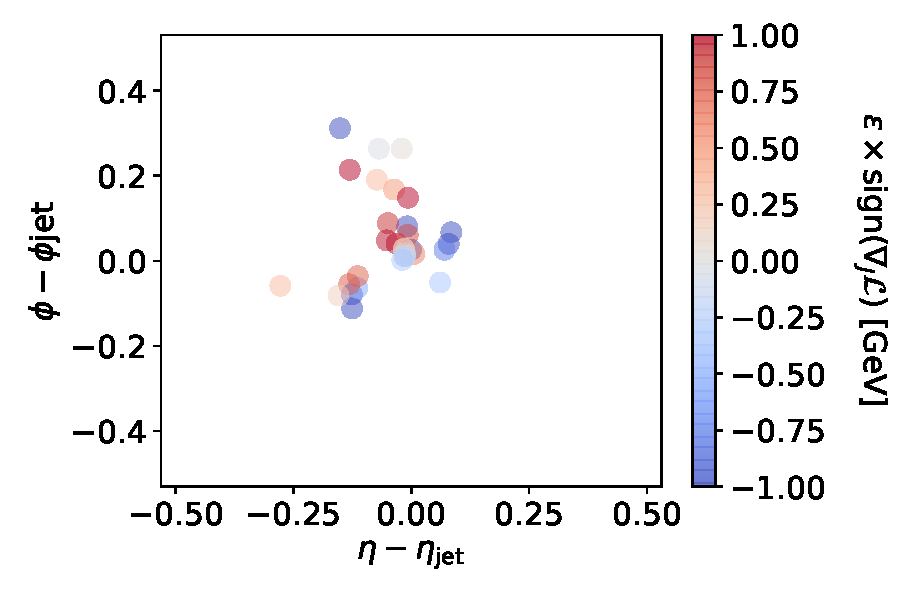
\includegraphics[width=0.15\textwidth]{figures/panel_3.pdf}
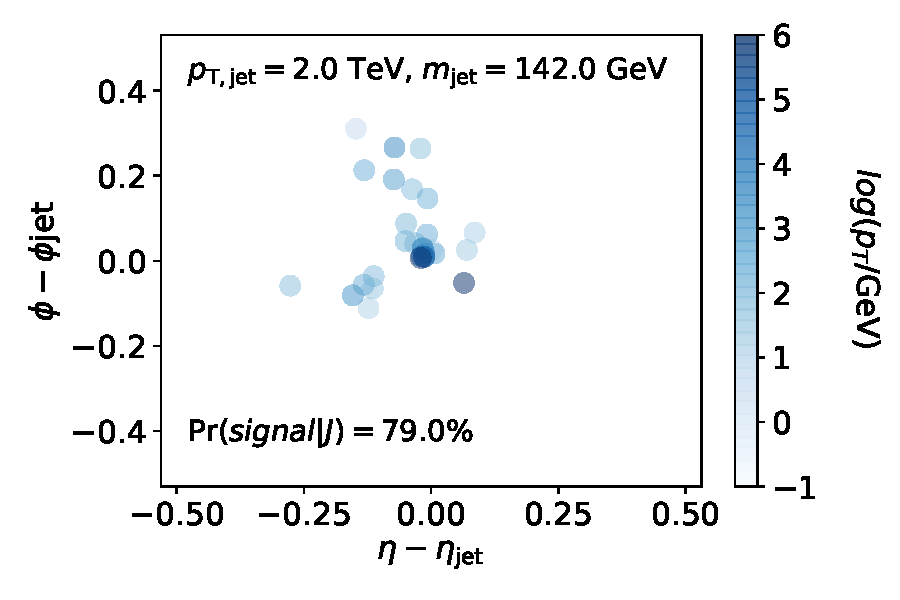
\includegraphics[width=0.15\textwidth]{figures/panel_2.pdf}
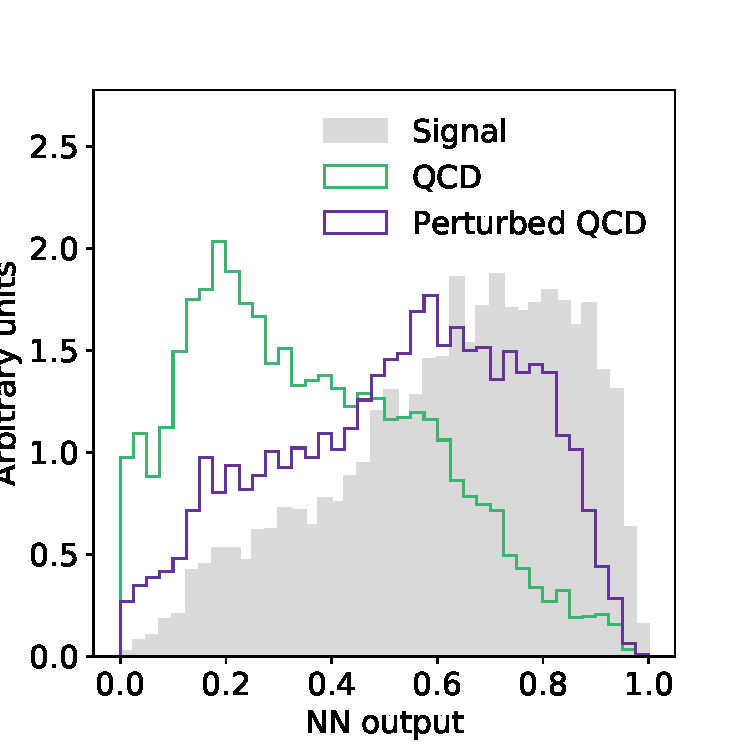
\includegraphics[width=0.23\textwidth]{figures/NN_FGSM.pdf}
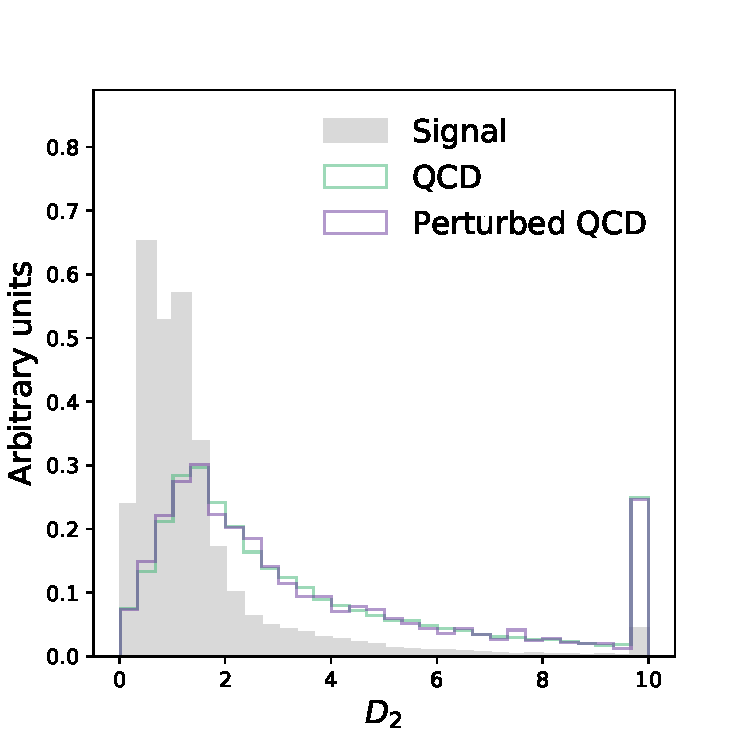
\includegraphics[width=0.23\textwidth]{figures/D2_FGSM.pdf}
\caption{The application of FGSM to jets.  The top row of plots show image representations of a single jet before (left) and after (right) an FGSM perturbation.  The grayscale indicates the particle $p_T$.  The middle plot illustrates the difference between the plots.  The lower plots show NN (left) and $D_2$ histograms for signal and background before and after the FGSM perturbation.  Both sets of jets are perturbed by the same amount, yet the distribution of $D_2$ is largely unchanged. }
\label{fig:FGSM}
\end{figure}

While the FGSM illustrated the sensitivity to small perturbations for single jets, it does not show how systematic ensemble perturbations could modify the classifier performance.  Blah...

\begin{align}
\label{eq:global}
g=\text{argmin}_{g'}\left[\mathcal{L}_\text{xe}(f(J+\delta J),\bar{y})+\mathcal{L}_\text{jet}(J,J+\Delta J)\right],
\end{align}

\section{Results}

\section{Conclusions}
Conclusions and outlook...

\section*{ACKNOWLEDGMENTS}

This work is supported by the DOE under contract DE-AC02-05CH11231. 

\bibliography{myrefs}

\end{document}